\section{Model-Free Prediction}
In Model-Free Prediction the objective is to estimate the value function of an \emph{unknown} MDP.

\subsection{Monte Carlo Methods}
In this section we consider our first learning methods for estimating value functions and discovering optimal policies. Here we \textbf{do not assume complete knowledge of the environment}. Monte Carlo methods require only \emph{experience} -- sequences of states, actions, and rewards from interaction with an environment.

\subsection{Monte Carlo Policy Evaluation (Prediction)}
Recall that the value of a state is the expected return starting from that state. An obvious way to estimate it from experience, then, is simply to average the returns observed after visits to that state. As more returns are observed, the average should converge to the expected value.

\begin{algorithm}
    \caption{First-visit MC prediction for estimating $V \approx v_\pi$}
    \begin{algorithmic}[1]
        \Loop
            \State Generate an episode following $\pi$: $S_0, A_0, R_1, S_1, A_1, R_2, \dots, S_{T-1}, A_{T-1}, R_T$
            \State $G \gets 0$
            \For{$t \gets T-1$ \textbf{downto} $0$}
                \State $G \gets \gamma G + R_{t+1}$
                \If{$S_t$ does not appear in $S_0, S_1, \dots, S_{t-1}$}
                    \State Append $G$ to $Returns(S_t)$
                    \State $V(S_t) \gets$ average($Returns(S_t)$)
                \EndIf
            \EndFor
        \EndLoop
    \end{algorithmic}
\end{algorithm}

When episodes are long learning can become slow because we have to wait till the end of an episode before actually learning anything useful.

\paragraph{First-visit vs.\ every-visit.} The algorithm above only records a return the
\emph{first} time a state is seen in an episode. The alternative, \emph{every-visit MC},
records a return \emph{every} time the state is visited within the same episode (so a
single episode can contribute multiple samples for the same state). Both converge to
$v_\pi$ as the number of visits $\to \infty$, but by slightly different arguments:
first-visit gives an i.i.d.\ sample of $G_t$ per episode;
every-visit samples are correlated within an episode, but the estimator is still
consistent and is more sample-efficient in practice.


\subsection{Temporal-Difference Learning}
Both TD and Monte Carlo methods use experience to solve the prediction problem. Given some experience following a policy $\pi$, both methods update their estimate $V$ of $v_\pi$. In general Monte Carlo methods
must wait until the end of the episode to determine the increment to $V(S_t)$
\[
    V(S_t) \gets V(S_t) + \alpha \left[ G_t - V(S_t) \right]
\]

Instead, TD methods need to wait only until the next time step: at time $t + 1$ they immediately form a target and make a useful update using the observed reward $R_{t+1}$ and the estimate $V (S_{t+1})$. The simplest TD method makes the update

\[
    V(S_t) \gets V(S_t) + \alpha [R_{t+1} + \gamma V(S_{t+1}) - V(S_t)]
\]

In effect, the target for the Monte Carlo update is the actual return $G_t$, whereas the target for the TD update is the estimate $R_{t+1} + \gamma V(S_{t+1})$.
\begin{itemize}
    \item $R_{t+1} + \gamma V(S_{t+1})$ is called \emph{TD Target}
    \item $\delta_t = R_{t+1} + \gamma V(S_{t+1}) - V(S_t)$ is called \emph{TD Error}
\end{itemize}

\begin{algorithm}
    \caption{Tabular TD(0) for estimating $v_\pi$}
    \begin{algorithmic}[1]
        \For{\textbf{each} episode}
            \State Initialize $S$
            \For{\textbf{each} step of episode}
                \State $A \gets$ action given by $\pi$ for $S$
                \State Take action $A$, observe $R, S'$
                \State $V(S) \gets V(S) + \alpha [R + \gamma V(S') - V(S)]$
                \State $S \gets S'$
            \EndFor
        \EndFor
    \end{algorithmic}
\end{algorithm}

Because TD(0) bases its update in part on an existing estimate, we say that it is a \emph{bootstrapping} method, like DP.

Monte Carlo methods use an estimate of $\mathbb{E}[G_t \mid S_t = s]$ as a target, whereas DP methods use an estimate of $\mathbb{E}[R_{t+1}+\gamma v_\pi(S_{t+1}) \mid S_t = s]$ as a target.
\begin{itemize}
    \item The Monte Carlo target is an estimate because the expected value is not known; a sample return is used in place of the real expected return.
    \item The DP target is an estimate not because of the expected values, which are assumed to be completely provided by a model of the environment, but because $v_\pi(S_{t+1})$ is not known and the current estimate, $V(S_{t+1})$, is used instead. 
\end{itemize}
The TD target is an estimate for both reasons: it samples the expected values, and it uses the current estimate $V$ instead of the true $v_\pi$.

\begin{table}[h]
    \centering
    \caption{Dynamic Programming vs.\ Monte Carlo vs.\ TD(0)}
    \begin{tabularx}{\linewidth}{l X X X}
    \toprule
     & \textbf{DP} & \textbf{MC} & \textbf{TD(0)} \\
    \midrule
    Model-free? & No & Yes & Yes \\
    Bootstraps? & Yes & No & Yes \\
    Waits for episode end? & N/A (full sweeps) & Yes & No \\
    Target & $\mathbb{E}[R + \gamma v(S')]$ & Return $G_t$ & $R + \gamma v(S')$ \\
    Bias & None & Unbiased & Biased \\
    Variance & None & High & Low \\
    Converges to & $v_\pi$ & min MSE to observed returns & max-likelihood Markov model \\
    Works in non-episodic tasks? & Yes & No & Yes \\
    \bottomrule
    \end{tabularx}
\end{table}


\subsection{Batch MC and TD}
Normally, in online RL, you update your value estimates immediately after experiencing a step or episode. In Batch Learning, you hold onto a fixed set of $K$ episodes and feed them to your algorithm repeatedly until the estimates converge.

Suppose you have $K=8$ episodes of experience structured like this:
\begin{align*}
    A,0, \quad B,0 \\
    B,1 \\
    B,1 \\    
    B,1 \\
    B,1 \\
    B,1 \\
    B,1 \\
    B,0
\end{align*}

What are $V(A)$ and $V(B)$? Obviously $V(B) = 6/8 = 0.75$, but for $V(A)$ we have two possible answers:
\begin{itemize}
    \item \textbf{Monte-Carlo:} $V(A)=0$ because the only time we saw $A$ happen the reward was $0$
    \item \textbf{TD(0):} $V(A) = V(B) = 6/8$ because every time $A$ happened we got to $B$, which has a value of $0.75$
\end{itemize} 
In general we have:
\begin{itemize}
    \item \textbf{MC} converges to the solution with minimum mean-squared error 
    \[
        \sum_{k=1}^{K} \sum_{t=1}^{T_k} (G_t^k - V(s_t^k))^2
    \]
    Where $G_t^k$ is the actual cumulative return observed from step $t$ until the end of episode $k$, $s_t^k$ is the state visited at step $t$ during episode $k$ and $V(s_t^k)$ is the current estimate for the value of state $s_t^k$
    \item \textbf{TD(0)} converges to the solution of maximum likelihood Markov Model
\end{itemize}

\subsection{n-step TD}
What is the space of methods lying between Monte Carlo and TD methods? Consider estimating $v_\pi$ from sample episodes generated using $\pi$. Monte Carlo methods perform an update for each state based on the entire sequence of observed rewards from that state until the end of the episode. The update of one-step TD methods, on the other hand, is based on just the one next reward, bootstrapping from the value of the state
one step later as a proxy for the remaining rewards.

One kind of intermediate method, then, would perform an update based on an intermediate number of rewards: more than one, but less than all of them until termination.

\begin{figure}[htbp]
    \centering
    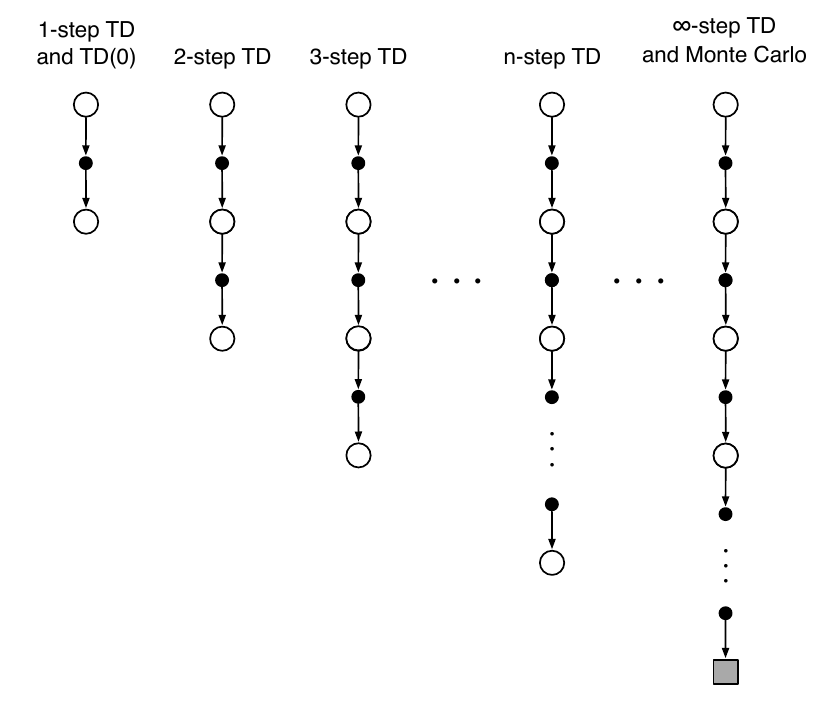
\includegraphics[width=0.3\textwidth]{figures/td_n_step.png}
\end{figure}

Consider the following $n$-step returns for $n=1,2, \dots, \infty$:
\begin{alignat*}{3}
    n &= 1      &\quad \textcolor{blue}{(TD)} &\quad G_t^{(1)}      &&= R_{t+1} + \gamma v(S_{t+1}) \\
    n &= 2      &\quad                        &\quad G_t^{(2)}      &&= R_{t+1} + \gamma R_{t+2} + \gamma^2 v(S_{t+2}) \\
      &\ \vdots &\quad \vdots                 &\quad                && \\
    n &= \infty &\quad \textcolor{blue}{(MC)} &\quad G_t^{(\infty)} &&= R_{t+1} + \gamma R_{t+2} + \dots + \gamma^{T-t-1} R_T
\end{alignat*}

So, in general, the $n$-step return is defined as:
\[
    G_t^{(n)} = R_{t+1} + \gamma R_{t+2} + \dots + \gamma^{n-1} R_{t+n} + \gamma^n V(S_{t+n})
\]

So, $n$-step TD learning can be calculated as:

\[
    V(S_t) \gets V(S_t) + \alpha \left( G_t^{(n)} - V(S_t) \right)
\]

\subsection{TD($\lambda$)}

Picking $n$ can be tough, and most certainly won't generalize to different environments, so let's find a way to avoid picking
altogether! We will do this by picking all different values of $n$ at once. How? The intuition is to average all the possible n-step returns into a single return. If we average these values in a smart way, we can do it super quick and still have something that intuitively makes sense.
Now we note that a valid update can be done not just toward any n-step return, but toward any average of n-step returns for different $n$-s. For example, an update can be done toward a target that is half of a two-step return and half of a four-step return: $\frac{1}{2}G_t^{(2)} + \frac{1}{2} G_t^{(4)}$.


\begin{figure}[htbp]
    \centering
    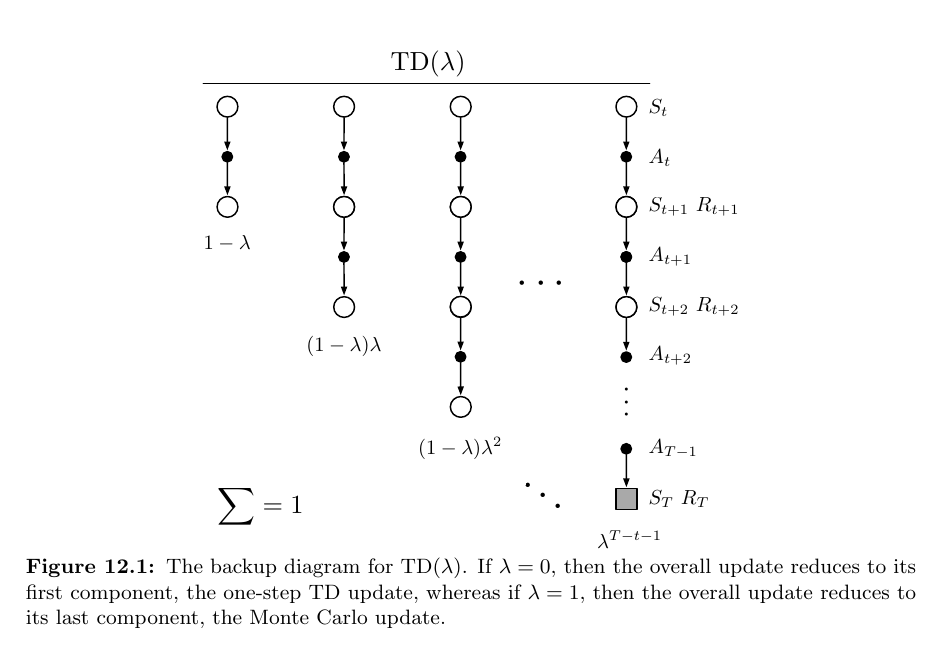
\includegraphics[width=0.5\textwidth]{figures/td_lambda.png}
\end{figure}

The $TD(\lambda)$ algorithm can be understood as one particular way of averaging $n$-step return $G_t^{(n)}$ using a weight that decays exponentially with time.  This average contains all the $n$-step updates, each weighted proportionally to $\lambda^{n-1}$ (where $\lambda \in [0, 1)$), and is normalized by a factor of $1-\lambda$ to ensure that the weights sum to 1. The resulting update is toward a return, called the $\lambda-return$, defined in its state-based form by:
\[
    G_t^\lambda \doteq (1-\lambda) \sum_{n=1}^{\infty} \lambda^{n-1} G_t^{(n)}
\]

The value function update for state $S_t$ then looks like a standard Monte Carlo update, but targeting $G_t^\lambda$:
$$V(S_t) \leftarrow V(S_t) + \alpha \left( G_t^\lambda - V(S_t) \right)$$

Note that to calculate $G_t^\lambda$ at time step $t$, you must wait until the episode finishes (or until far into the future) to collect $R_{t+1}, R_{t+2}, \dots, R_T$.

The approach that we have been taking so far is what we call the theoretical, or \emph{forward}, view of a learning algorithm. For each state visited, we look forward in time to all the future rewards and decide how best to combine them. We might imagine ourselves riding the stream of states, looking forward from each state to determine its update.

\begin{figure}[htbp]
    \centering
    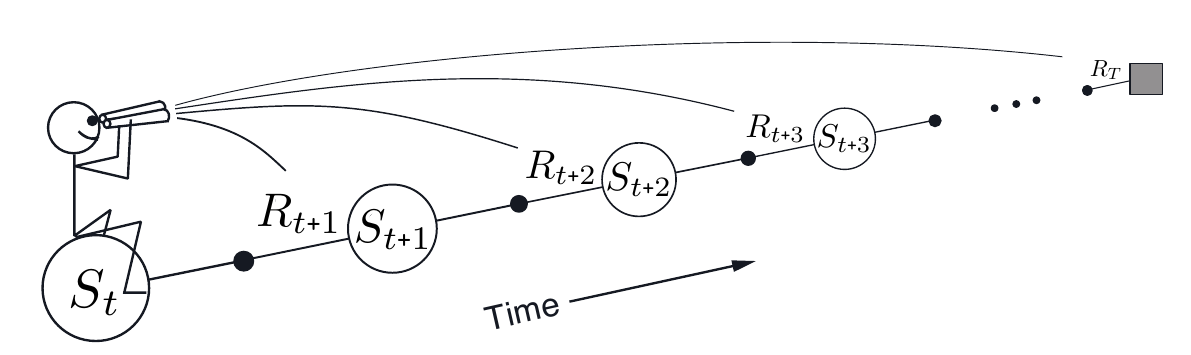
\includegraphics[width=0.5\textwidth]{figures//forward_view.png}
\end{figure}

After looking forward from and updating one state, we move on to the next and never have to work with the preceding state again. Future states, on the other hand, are viewed and processed repeatedly, once from each vantage point preceding them.

\subsection{Eligibility Traces}
We can clearly see that $TD(\lambda)$ with forward view has the same issues as Monte-Carlo: we have to wait until the episode ends to actually learn something. That's why \emph{backward} view was introduced: while forward view provides the theory, the backward view provides the actual mechanism used. But before going there we have to dive into the important concept of \textbf{eligibility traces}. Here, instead of waiting for what is going to happen next to be able to perform an update, we will remember what happened in the past and use current information to update the state-values for every state we've seen so far.

Let's start with a simple example: imagine you're a mouse going after a piece of cheese but, when you're nearing it, you hear a bell three times, a light comes on and you get electrocuted. Now: did the mouse get electrocuted because of the bell (most \emph{frequent} occurring state) or because of the light (most \emph{recent} occuring state)? Eligibility traces combine both the frequency and recency heuristics:
\begin{align*}
    E_0(s) &= 0 \\
    E_t(s) &= \gamma \lambda E_{t-1}(s) + \mathbbm{1}(S_t=s) \quad \forall \, s \in \mathcal{S}
\end{align*}

The idea is that every time we visit the state $S_t = s$ we increase the eligibility traces by adding $+1$. As we start not visiting that state anymore, the eligibility traces decay exponentially.

So now we can actually introduce the \emph{backward} view $TD(\lambda)$ algorithm: we keep an eligibility trace for every state $s$ then we update the value $V(s)$ for every state $s$ in proportion to the TD-error $\delta_t$ and eligibility trace $E_t(s)$:
\begin{align*}
    \delta_t &= R_{t+1} + \gamma V(S_{t+1}) - V(S_t) \\
    V(S) &\gets V(S) + \alpha \delta_t E_t(S)
\end{align*}

\begin{figure}[htbp]
    \centering
    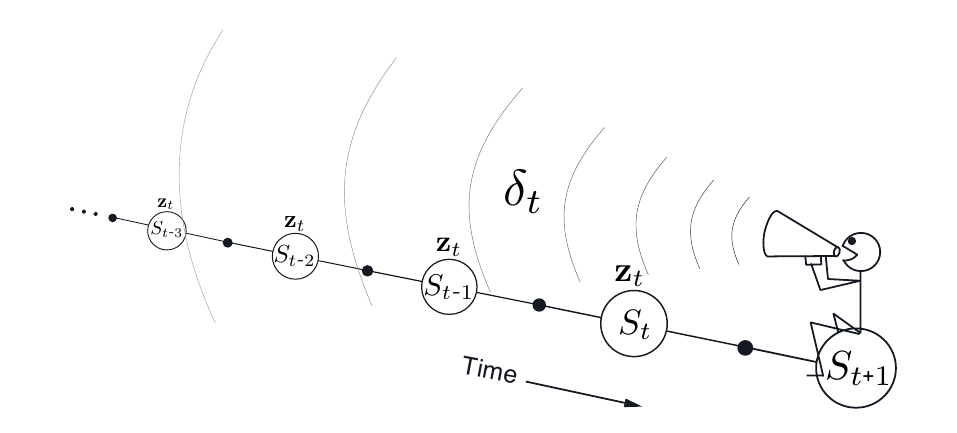
\includegraphics[width=0.5\textwidth]{figures//backward_view.png}
\end{figure}

So now we're no longer looking into the future, but instead we sort of "broadcast" this TD-error backwards to every state in the past, and the value function at each of those states is updated in proportion to the TD-error.

\paragraph{TD($\lambda$) and TD(0)}
When $\lambda = 0$, only the current state gets updated, so:
\begin{align*}
    E_t(s) &= \mathbbm{1}(S_t=s) \\
    V(s) &\gets V(s) + \alpha \delta_t E_t(s)
\end{align*}
Which is exactly equivalent to the TD(0) update $V(S_t) \gets V(S_t) + \alpha \delta_t$

\begin{table}[htbp]
    \centering
    \caption{Forward vs.\ Backward View of $\text{TD}(\lambda)$}
    \begin{tabularx}{\linewidth}{l X X}
    \toprule
     & \textbf{Forward view} & \textbf{Backward view} \\
    \midrule
    What it computes & $\lambda$-return $G_t^\lambda$ & Eligibility trace $E_t(s)$ \\
    \addlinespace
    When can you update? & Only at episode end & Every timestep \\
    \addlinespace
    Role & Theoretical target & Online mechanism \\
    \addlinespace
    Equiv.\ to TD(0) when & $\lambda = 0$ & $E_t(s) = \mathbbm{1}(S_t = s)$ \\
    \addlinespace
    Equiv.\ to MC when & $\lambda = 1$ & Trace decays only by $\gamma$, never by $\lambda$ \\
    \bottomrule
    \end{tabularx}
\end{table}